\documentclass[a4paper]{scrreprt}

\usepackage[german]{babel}
\usepackage[left=2cm, right=2cm, top=2cm, bottom=3cm]{geometry}
\usepackage{fancyhdr}
\usepackage{LastPage}
\usepackage{booktabs}
\usepackage{siunitx}
\usepackage{pgfplotstable}
\usepackage{microtype} % helps with justification
\usepackage{graphicx}
\usepackage{float}
\usepackage{hyperref}

\title{OOP1 Dokumentation}
\subtitle{Referenzverwaltung}
\date{\today{}}
\author{Rafael Stauffer}

\DeclareRobustCommand{\filename}{
Stauffer Rafael OOP1 Dokumentation.pdf
}

\pagestyle{fancy}
\fancyhf{}
\lfoot{\filename}
\rfoot{Seite \thepage\phantom{x}von \pageref{LastPage}}

\begin{document}
\maketitle{\thispagestyle{fancy}}
\tableofcontents{\thispagestyle{fancy}}
\section{Versionierung}
\begin{table}[h!]
\begin{center}
\pgfplotstabletypeset[col sep=comma,
display columns/0/.style={column name=$Datum$,string type,column type/.add={|}{|}},
display columns/1/.style={column name=$Name$,string type},
display columns/2/.style={column name=$Beschreibung$,string type,column type/.add={|}{|}},
every head row/.style={before row={\toprule},after row={\midrule},},
every last row/.style={after row=\bottomrule},]{versionierung.csv}
\end{center}
\end{table}
\newpage
\section{Zusammenfassung}
\subsection{Bedienung}
{\large Quellen und Referenzen verwalten, jetzt neu bequem in JavaFX.\\}

Übersichtsfenster über den Menüpunkt View wechselbar.\\
Einträge über den Menüpunkt Edit verwalten oder bequemer mit den Schnelltasten:
\begin{itemize}
	\item Doppelklick oder Enter auf existierendem Objekt: Gewähltes Objekt bearbeiten.
	\item Doppelklick auf leere Zeile: Neues Objekt erstellen.
	\item Delete: Gewähltes Objekt löschen.
\end{itemize}

\begin{figure}[H]
	\centering
	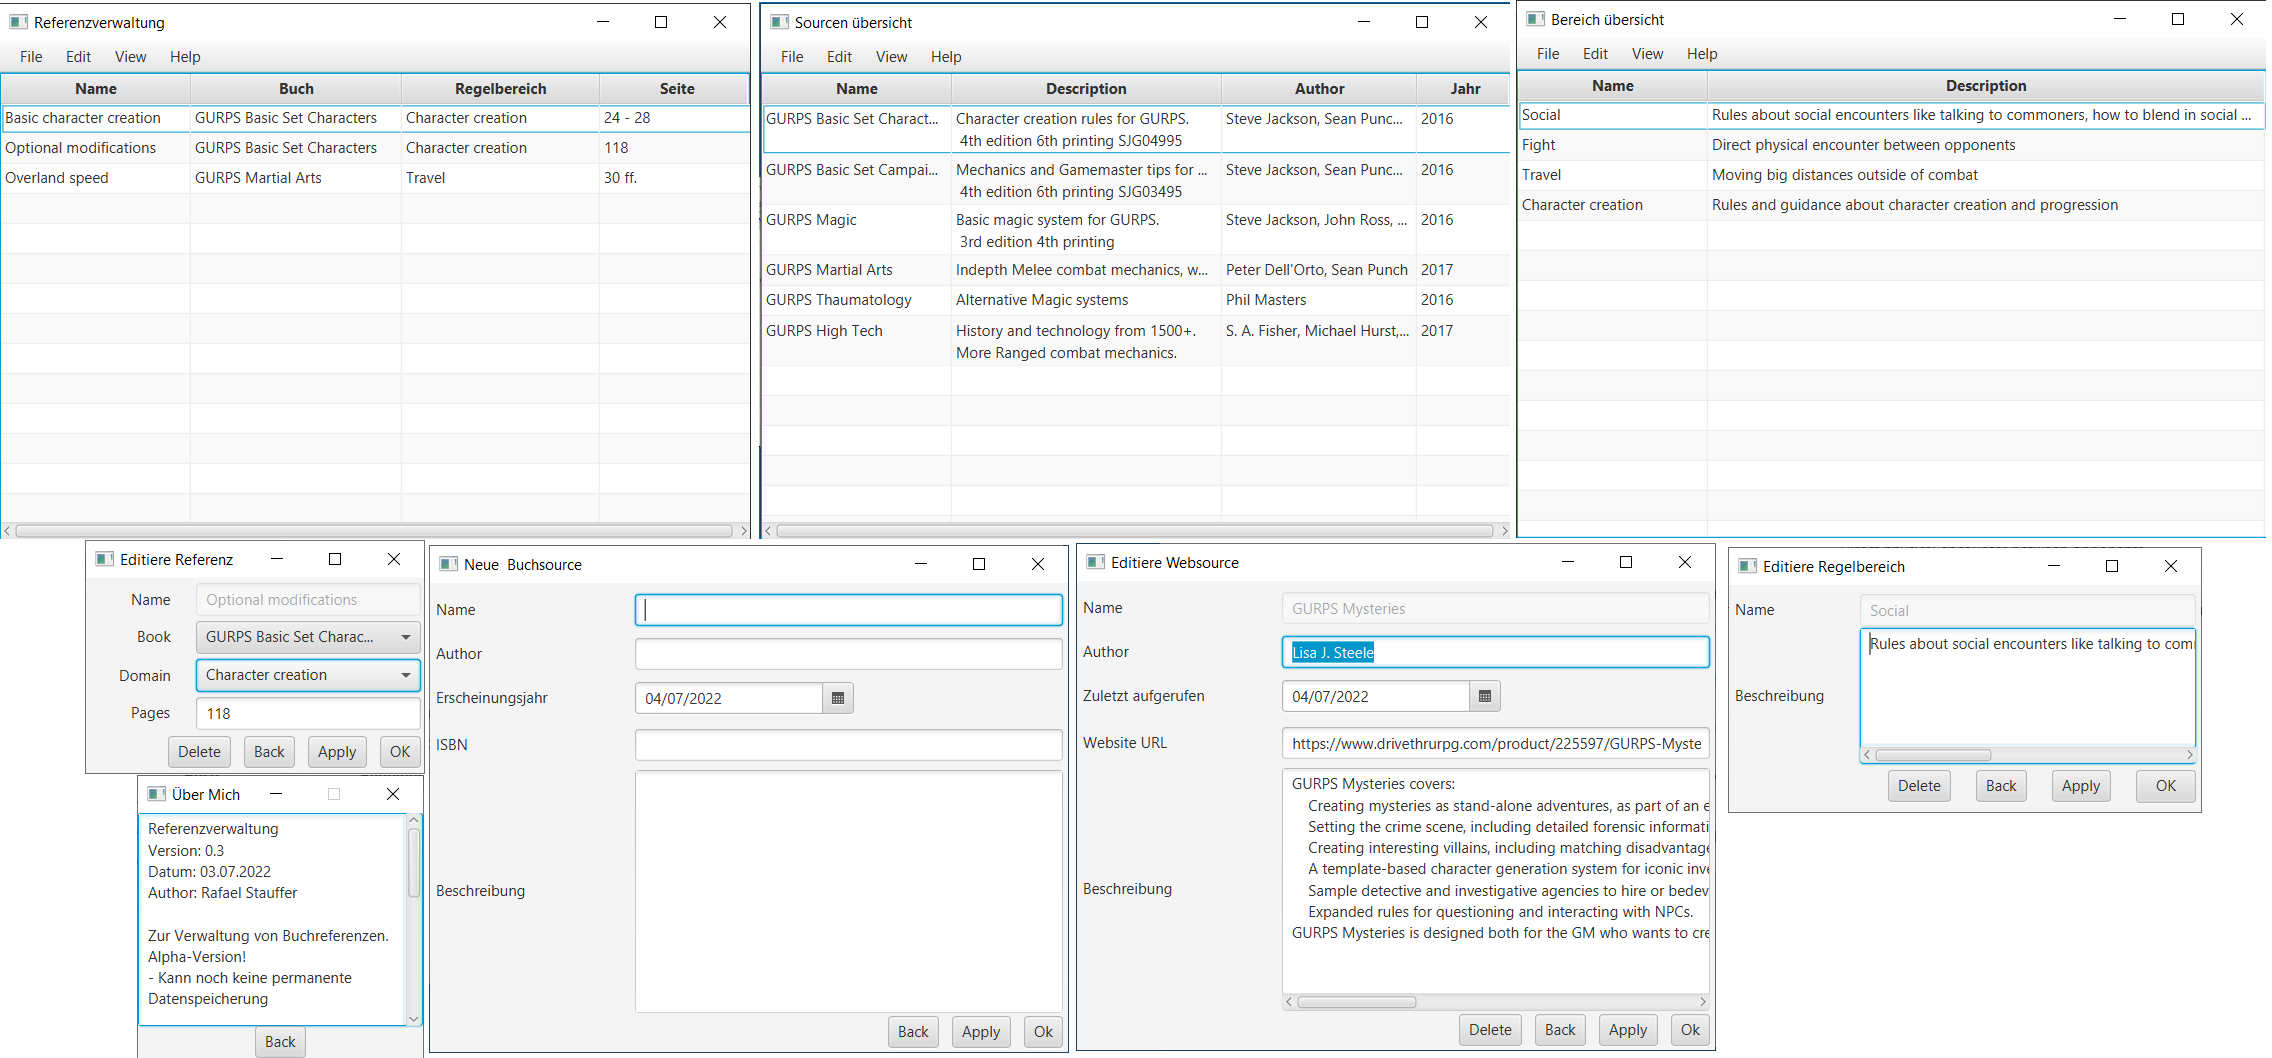
\includegraphics[width=0.95\textwidth]{screenshots}
	\caption{Alle Fenster im Überblick.\\{\footnotesize Von links oben im Uhrzeigersinn: Referenzübersicht-Hauptfenster, Sourcenübersicht, Bereichsübersicht, Bereich-Detailfenster im Editiermodus, Website-Detailfenster im Editiermodus, Buch-Detailfenster im Erstellmodus, ÜberMich-Infofenster, Referenz-Detailfenster im Editiermodus}}
\end{figure}

\subsection{Git}

Das Projekt ist unter \url{https://dev.hftm.ch:4430/rafael.stauffer/oop1-projektarbeit} gespeichert.\\
Wie im ReadMe beschreiben kann das maven verzeichnis per {\ttfamily mvn clean javafx:run} direkt ausgeführt oder per {\ttfamily mvn clean compile package} in ein JAR kompiliert werden welches sich unter {\ttfamily /maven/target/Referenzverwaltung-0.3-SNAPSHOT.jar} befindet.

\subsection{Code Architektur}

Im total existieren acht Controller-Klassen mit je einer dazugehörigen View welche von der BaseController-Basisklasse abgelietet werden.
Die drei Overview-Klassen sind für die jeweiligen Tabellenübersichten zuständig. Die vier Detail-Klassen verwalten die Erstell- und Bearbeitungs-formulare. Der AboutController verwaltet das ÜberMich-Fenster.

\begin{figure}[H]
	\centering
	
\includegraphics[width=0.95\textwidth]{controller}
	\caption{Controller-Klassen}
\end{figure}

Business-Daten wurden wie im Szenarienbeschrieb definiert in drei Klassen gespeichert, dabei wurde aber die Source-Klasse weiter in SourceBook (mit Erscheinungsjahr und ISBN) und SourceWeb (mit URL und letztem Seitenaufruf) unterteilt.

\begin{figure}[H]
	\centering
	
\includegraphics[width=0.95\textwidth]{business_klassen}
	\caption{Business-Objekte und DataAccessObject}
\end{figure}
\newpage
\section{Funktionen}
\subsection[Funktion 1 Objektklassen]{Funktion 1 Im Minimum eine Objekt Klasse erstellt.}

\subsubsection{Anforderung}
In der Konzept-Phase beim Szenarienbeschrieb wurden drei Business-Object-Klassen identifiziert:
\begin{itemize}
	\item Buch
	\item Referenz
	\item Regelbereich
\end{itemize}

\subsubsection{Design}
Durch das Proof of Concept für die BibTex-Dokumente wurden die Business-Object-Klassen mit der unterscheidung von Buch und Website auf vier erweitert.\\
Ein weiteres normalisieren der Daten auf Author wurde wegen dem Projektumfang verworfen. Interfaces zu den in der Anforderung definierten Objekten wurden für die zukünftige Flexibilität miteinbezogen. Sämtliche Attribute wurden zur Einfachheit als Strings festgelegt.
\begin{itemize}
	\item BuchSource
	\item WebsitenSource
	\item Referenz
	\item Regelbereich
\end{itemize}

\subsubsection{Entwicklung}
Umsetzung wie nach Design. Erste Version nur Referenz mit Source und Regelbereich als Dummy-Objekt zum Testen bevor die Vollständige funktionalität umgesetzt wurde. Nach dem ersten Prototypen wurden Einschränkungen der 'jedes Attribut ein String' Methodik sichtbar. Zur besseren Überprüfung der Eingaben und Zukunftsicherheit wurde das Erscheinungsjahr/LetzterAufruf-Feld als LocalDate definiert welches einfacher dem DatePicker übergeben werden kann. Website wurde als URL definiert was kurzzeitig für Probleme bei der Übergabe an die View gesorgt hat aber ungültige URLs automatisch erkennt. Ursprünglich wurde eine Persistenz der Daten eingeplant aber wegen dem Projektumfang verworfen und stattdessen das DataAccessObject-Pattern eingebaut um diese zukünftig nachzuliefern.

\subsubsection{Test}
Zusammen mit Funktion 3 getestet. Alle Objekte wurden wiederholt erstellt, geändert und gelöscht. 

\subsubsection{Fazit}
Die Vererbung und Interfaces könnten eleganter gelöst sein. Der bisherige Aufbau stellt ein Kompromiss zwischen Aufwand/Projektumfang und Erweiterbarkeit dar.
\subsection[Funktion 2 JavaFX GUI]{Funktion 2 JavaFX als grafische Oberfläche eingesetzt mit mindestens 2 Views}

\subsubsection{Anforderung}

Der Szenarienbeschrieb beinhaltet drei Paare mit je einem Übersichts- und einem Detail-Screen im Total sechs Views.

\subsubsection{Design}

Für die Übersichts-Screens wurden ListViews geplant um eine einfache Ansicht in einem minimalistischen Design bereitzustellen mit Änderungs und Löschfunktionen direkt auf der Zeile.
Die Detail-Screens wurden als Erstellungs- und Bearbeitungs-Screen geplant welche je nach Aufruf Nodes ein- oder ausblenden aufgebaut auf VBox/HBox und Textboxen. Es wurde noch nicht festgelegt ob die Detail-Screens in einem neuen Fenster/Stage erscheinen oder die aktuelle Stage übernehmen sollten.

\subsubsection{Entwicklung}
Beim der Entwicklung des Referenz-Screen-Paars wurde klar, dass:
\begin{itemize}
	\item die ListView zu unflexibel ist für die verschiedenen Business-Objekte: TableViews stattdessen verwendet
	\item VBox/HBox-Verschachtelungen die Detail-Screens nur bedingt darstellen können: GridPanes wurden stattdessen verwendet
	\item die Stage übernahme des Detail-Screens vom Übersichtscreens die komplexität erhöht ohne grosse Vorteile: Detail-Views starten somit in eigener Stage
	\item die Views immer etwa gleich aufgebaut sind: eine BaseController-Klasse wurde eingeführt
	\item SubViews die Komplexität massiv erhöhen: keine SubScreens verwendet
\end{itemize}
Obwohl weitere Entkoppelungen der Nodes besonders im Overview-Screen möglich sind wurden diese wegen Zeitdruck nicht umgesetzt.

\subsubsection{Test}
\begin{itemize}
	\item Starten und Beenden der Views in eigenen Stages.
	\item Starten und Beenden der Views in Parent Stage.
	\item Parameterübergabe zwischen Controller.
	\item Aufruf von Events.
	\item Verändern von View-Feldern.
	\item Vererbung von Event und Feldverknüpfungen
\end{itemize}

\subsubsection{Fazit}
Die Arbeit mit FXML war besonders ermüdend, da kaum Debugginginformationen weitergereicht wurden.
\subsection[Funktion 3 CRUD]{Funktion 3 Ein Objekt muss erstellt, geändert und gelöscht werden können}

\subsubsection{Anforderung}
Sourcen, Bereiche und Referenzen müssen verwaltet werden können. Dabei wurde festgelegt, dass Bereiche und Sourcen nur gelöscht werden können, wenn sie nicht von Referenzen aktiv verwendet werden können.

\subsubsection{Design}
Ein DataAccesssObject (DAO) als Singleton wurde gewählt um die Datenverarebeitung von der Datenspeicherung zu lösen. Eine Serialisierung in einzelne lokale Dateien zur Persistierung der Daten wurde eingeplant. Das DAO soll interne Arrays halten welche von den Controllern abgefragt und als ObservableList weiterverwendet werden können. In der Referenz sind der Bereich und die Source als Objektreferez gespeichert und werden über diese Abgefragt.

\subsubsection{Entwicklung}
DAO wurde geändert sodass direkt ObservableLists darin verwaltet werden welche nur noch von den Controllern referenziert werden. Dies vereinfacht das Event-Handling bei Erstellung und Löschung. Die Persistierung der Daten wurde wegen zu hohem Aufwand nicht durchgeführt. Die Source und Bereich sind weiterhin als Objektreferenzen in der Referenz gespeichert, jedoch wird primär der jeweilige Name zur Verknüpfung verwendet um die Objekte zu entkoppeln. Dies aber verbietet die Bearbeitung des Namens, da dieser nun den Primärschlüssel darstellt.

\subsubsection{Test}
\begin{itemize}
	\item Erstellen einer Referenz/Source/Bereich
	\item Ändern eines Referenz/Source/Bereich
	\item Löschen eines Referenz/Source/Bereich
	\item Testen der Lösch-Verhinderung einer Source/Bereich welche verwendet wird
	\item Testen der Änderungs-Verhinderung eines Namens bei bereits erstelltem Objekt
	\item Referenzieren einer neu erstellten Source/Bereich in einer Referenz
	\item Übernahme der Veränderung vom Detail-Screen in die Übersichtstabelle
\end{itemize}

\subsubsection{Fazit}
Die Verbindung zwischen ObservableList und den Tabellen war ein Knackpunkt, da Änderungen an Objekt-Attributen nicht zuverlässig weiterkommuniziert wurden. Als Umgehungslösung werden bei einer Änderung die Objekte gelöscht und neu in die ObservableList eingefügt, dabei werden vorhandene Verknüpfungen neu erstellt.
\subsection[Funktion 4 Menü]{Funktion 4 Einsatz eines Menüs auf der grafischen Oberfläche mit den Menüitems Über mich und Exit.}

\subsubsection{Anforderung}
Der Szenarienbeschrieb selbst hat keine weiteren Anforderungen an das Menü gestellt.

\subsubsection{Design}
Ein Menü mit den geforderten Menüitems sowie eines Kapitels Edit für die CRUD-Operationen und View zum wechseln in die anderen Übersichtsbereiche wurde geplant. Eine View nur mit dem Menü welches danach dynamisch über dem Inhalt angezeigt wird wurde geplant.

\subsubsection{Entwicklung}
Die View-Platzierung hat nicht funktioniert und es wurde stattdessen das Menü in jedes Übersichts-View eingefügt. Diese Lösung ist von geringer Wiederverwendbarkeit hat aber die Entwicklung und spezifische Anpassung des Sourcen-Menüs beschleunigt.

\subsubsection{Test}
\begin{itemize}
	\item Exit schliesst alle Fenster
	\item ÜberMich öffnet Informationsfenster
	\item Edit-MenüItems starten entsprechende CRUD-Operationen
	\item View-MenüItems wechseln zum entsprechenden Übersichtsfenster
\end{itemize}

\subsubsection{Fazit}
Bis auf das SubScreen-Problem ging die Entwicklung rasch voran und das Entwerfen des Menülayouts im SceneBuilder war einfach.
\subsection[Funktion 5 Listeneinsatz mit Beispielobjekten]{Funktion 5 Einsatz einer Liste sowohl im Controller auch als auf der grafischen Oberfläche und es müssen mindestens drei Beispielobjekte beim Starten in die Liste eingetragen werden.}

\subsubsection{Anforderung}
Für jede der drei Objekten (Source, Referenz und Bereich) wurde je eine Übersichtsliste auf der Oberfläche und eine dazugehörige Liste im Controller geplant.

\subsubsection{Design}
Ausgabe auf der Oberflächer wurde per ListView geplant, dahinter im Controller die dazugehörige ObservableList welche vom DataAccessObject (DAO) aus einem Array gespeist wird.

\subsubsection{Entwicklung}
Für die Übersicht und Sortierung wurde die ListView durch eine TableView ersetzt. Die ObservableLists werden direkt vom DAO verwaltet. Nur in Sonderfällen wie die Verknüpfung von der Referenz mit Source/Bereich muss der Controller selbst die Liste verwalten. Beim Instanzieren des DAO werden die Beispielobjekte in die jeweiligen Listen instanziert.

\subsubsection{Test}
\begin{itemize}
	\item drei oder mehr Beispielreferenzen in Referenzübersicht vorhanden
	\item drei oder mehr Beispielsourcen in Sourceübersicht vorhanden
	\item drei oder mehr Beispielbereiche in Bereichübersicht vorhanden
	\item Befüllung der Source- und Bereich-ComboBox beim Erstellen und Bearbeiten einer Referenz
\end{itemize}

\subsubsection{Fazit}
Das Arbeiten mit den TableViews und ObservableLists war einfach. Einzig die Erstellung der CellValueFactory und RowFactory zur Formatierung und Event-Handling benötigte erwas einarbeitszeit.
\subsection[Funktion 6 Alerts]{Funktion 6 Verwendung von Alerts bei Benutzereingaben}

\subsubsection{Anforderung}
Pflichtfender wie Name müssen ausgefüllt werden, Fehlermeldung beim Löschversuch von Referenzierten Sourcen/Bereichen und Überprüfung der Eingabe wie zB: ISBN Nummer benötigen Alerts als Nutzerfeedback.

\subsubsection{Design}
In der Design-Phase wurde festgelegt, dass nur Error-Fehlermeldungen und JaNein-Fragen verwendet werden. In diesem limitierten Umfang gibt es keine Verwendung für Info-Meldungen oder Warnungen. Zur wiederverwendbarkeit wurden diese beiden Fälle in dem BaseController abgebildet.

\subsubsection{Entwicklung}
Einbau in den BaseController zur wiederverwendbarkeit, zur einfachen Handhabung in den einzelnen Controllern wurde die komplexe Rückgabe des JaNein-Dialogs auf ein simples boolean (true = Ja, false = alles andere) reduziert. Diese Methode askYesNo konnte damit an allen drei Lösch-Funktionen einfach wiederverwendet werden. Ebenfalls wurde die Methode showError 14 mal wiederverwendet um die einzelnen Eingabefehler rückzumelden.

\subsubsection{Test}
\begin{itemize}
	\item JaNein-Dialog wird beim Löschen angezeigt
	\item Objekt wird nur bei der Wahl Ja gelöscht im JaNein-Dialog
	\item JaNein-Dialog zeigt Name des zu löschenden Objekts an
	\item Bei Fehlendem Name wird ein Error-Dialog angezeigt und nicht gespeichert
	\item Bei fehlerhaften ISBN wird ein Error-Dialog angezeigt und nicht gespeichert
	\item Bei fehlerhaften URL wird ein Error-Dialog angezeigt und nicht gespeichert
\end{itemize}

\subsubsection{Fazit}
Nach kurzem Durchlesen der Dokumentation über Alerts waren diese einfach zu benutzen.
\subsection[Funktion 7 Selektion]{Funktion 7 Einsatz mindestens einer Variante der Selektion im Controller}

\subsubsection{Anforderung}
Selektionen werden beim Eingabeprüfung getroffen werden um dem Nutzer Feedback zu geben.

\subsubsection{Design}
Es wurde dieser Anforderung keine nähere Design-Betrachtung geschenkt, da sich eine gelgenheit für eine Selektion finden würde in diesem mässig komplexen Projekt.

\subsubsection{Entwicklung}
Nutzereingabenprüfung wurde in die checkInputData-Methoden der DetailController implementiert welche eine Serie von IfElse-Selektionen verwenden um die Daten zu validieren. Einzig im DataAccessObject in der Methode checkIsbnValid wurde ein SwitchCase verbaut, da es sich dort auf die Vorgehensauswahl anhand der ISBN-Länge angeboten hat.

\subsubsection{Test}
Korrekte Funktion der Selektionen wurde im Rahmen von F6 Alerts überprüft.

\subsubsection{Fazit}
Einfache implementation. Auf die Verwendung von equals bei Stringvergleichen muss geachtet werden.
\subsection[Funktion 8 Iteration]{Funktion 8 Einsatz minestens einer Variante der Iteration im Controller}

\subsubsection{Anforderung}
Das Befüllen der Listen hat sich hier angeboten.

\subsubsection{Design}
Das initiale Design plane die ArrayList der Objekte vom DataAccessObject (DAO) im Controller per for-Loop in eine ObservableList umzuwandeln.

\subsubsection{Entwicklung}
Durch die Änderung der Architektur (siehe F3) wie die Listen direkt im DAO verwaltet werden entfällt die initial geplante Iteration im Controller. Einzig der RefDetailController enthält noch Schleifen welche die Sourcen und Bereiche in die ComboBoxen füllen. Alle komplexeren Schleifen wurden in das DAO ausgelagert wie zB: checkIsbn10 und checkIsbn13 welche die Prüfsummen der ISBN-Nummern berechnen und validieren.

\subsubsection{Test}
Korrekte funktion der Iterationen wurde in F3, F5 und F6 validiert.

\subsubsection{Fazit}
Einfache implementation wobei die forEach-Iteration der klassischen for-Iteration und while-Iteration mit Integer-Iterator vorgezogen wurde da sie eine kürzere und sicherere Schreibweise besitzt.
\subsection[Funktion 9 Methode im Controller]{Funktion 9 Im Controller minestens eine Methode eingesetzt.}

\subsubsection{Anforderung}
Methoden wurden nicht besonders in der Anforderung beachtet, da durch die Quellcodestrukturierung zur Übersichtlichkeit und Wiederverwendbarkeit autmatisch Methoden eingesetzt werden.

\subsubsection{Design}
Zur Eingabevalidierung wurden in den Detailcontroller die Methoden checkInputData und zur Generierung des Objektes aus den Feldern getDomainFromFields/getSourceFromFields/getReferenceFromFields implementiert. Wiederverwendbare Methoden befinden sich im BaseController. Objektmanipulation im DataAccessObject (DAO) oder den Objekten selbst.

\subsubsection{Entwicklung}
Methoden wurden iterativ ausgearbeitet, wann immer ein Codeteil mehrmals wiederverwendet werden konnte ohne weitere Komplexität zu addieren wurde daraus eine Methode erstellt. Dies ist sehr gut im BaseController beobachtbar wo die drei Übersichtsszenen immer mit der gleichen Methode showSceneOnStage aufgerufen werden, da sie sich identisch verhalten. Die Detailszenen werden trotz grosser Code überschneidung durch verschiedene Methoden aufgerufen, da für das Refaktorieren in eine Methode weitere Hilfsstrukturen eingefügt werden müssten.

\subsubsection{Test}
Methoden wurden passiv durch die anderen Funktionstest geprüft.

\subsubsection{Fazit}
Die Vorgehensweise war nicht sehr strukturiert und manche Methoden welche in einer Iteration entwickelt wurden konnten in der nächsten bereits wieder verworfen werden (zB: update Methoden der Business-Objekte von F1 werden nicht verwendet, da das Event-Handling nicht darauf abgestimmt ist, dies wurde aber erst nach der Implementation dieser geprüft).

\end{document}